% !TEX root = main.tex
\section{Systemüberblick}
\label{sec:system}
In diesem Abschnitt wird die Systemstruktur gezeigt, sowie alle, zur Build- und Runtime relevanten Komponenten von GraalVM NativeImage erläutert.

Der Anwendungscode (Java Bytecode), die benötigten Bibliotheken, das JDK und VM-Komponenten(SubstrateVM)\footnote{Umfasst u.A. Speicherverwaltung, Thread-Scheduling und Garbage Collection} dienen als Eingabe des sog. \textit{image builders}. Dieser verarbeitet die Eingabe und produziert daraus eine, auf ein spezifisches Betriebssystem und Prozessorarchitektur angepasste, nativ ausführbare Datei, ein \textit{native image}. 
Abbildung \ref{fig:system_buildtime} zeigt die Komponenten und den Ablauf des Build-Vorgangs eines \textit{native image}.

\begin{figure}[ht]
	\centering
	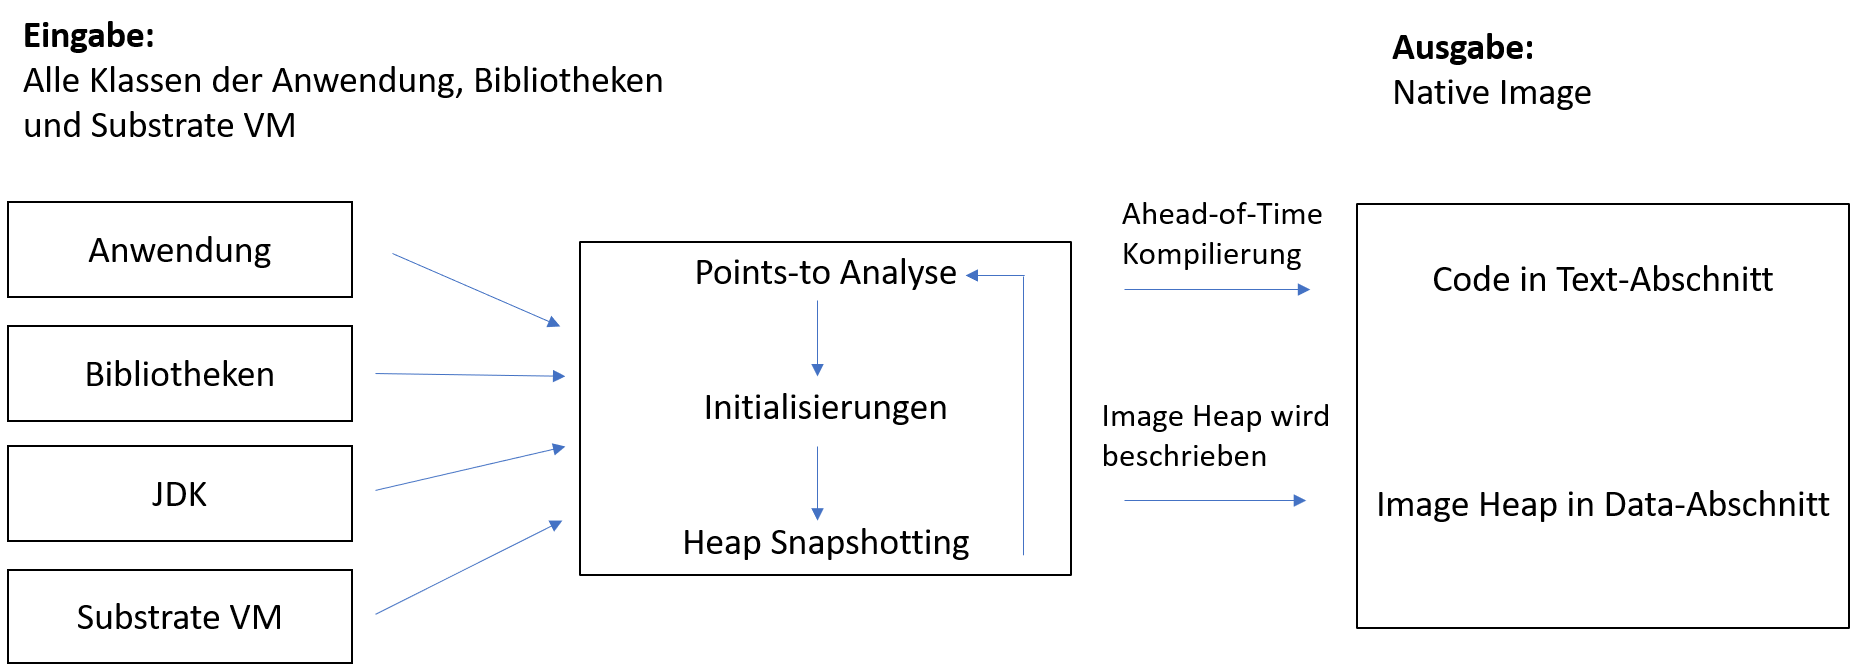
\includegraphics[width=1\textwidth]{resources/GraalVM_BuildTime.png}
	\caption{NativeImage Build-Vorgang}
	\label{fig:system_buildtime}
\end{figure}

Auf der Eingabe werden die Points-To Analyse, das Ausführen von Initialisierungscode und das Heapsnapshotting iterativ durchgeführt bis ein definierter Punkt erreicht ist. 
Zudem werden die registrierten Callbacks der Anwendung, die über die Feature-API von GraalVM nutzbar sind, in diesem Zuge auch ausgeführt. Das Ergebnis dieses Prozesses ist eine Liste von, zur Laufzeit, erreichbaren Klassen, Methoden und Feldern, sowie ein Objekt-Graph mit erreichbaren Objekten. Im Letzten Schritt des Build-Vorgangs werden die erreichbaren Methoden zu Maschinencode kompiliert und der Objekt-Graph wird als \textit{image heap} ausgeschrieben, und in die Form des zur Laufzeit tatsächlich vorhandenen Heaps transformiert. Danach wird der Maschinencode 
 in die Text-Section, und der image heap in die Data-Section \parencite[Fig. 1-13]{TISC1995} des native image geschrieben. Der gesamte Prozess wird \textit{image build time} genannt\parencite{Wimmer2019}.
Der \textit{image builder} selber ist eine Java-Anwendung. Sowohl die Pointer-Analyse 
und das ahead-of-time-Compiling, als auch das Ausführen der Klasseninitializer und Callback-Funktionen, werden also von ein und derselben JVM
 übernommen\textit{}.\footnote{Das heißt wiederrum, dass bei der \textit{image build time}, die Objekte, aus denen sich der spätere \textit{image heap} zusammensetzt,
 normale Objekte im Java Heap des \textit{image builder} sind.}
